\documentclass[a4paper,12pt]{article}
\usepackage[T1]{fontenc}
\usepackage[utf8]{inputenc}
\usepackage[english,russian]{babel}
\usepackage{pdfpages}
\usepackage{amsmath,amsfonts,amssymb,amsthm,mathtools}
\usepackage[left=10mm, top=10mm, right=10mm, bottom=20mm, nohead, nofoot]{geometry}
\usepackage{wasysym}
\author{\LARGEМерзляков Арсений}
\title{Анализ функции}
\pagestyle {empty}
\begin{document}
\maketitle
\begin{flushleft}
\Large
$f(x) = \sin {(x)} \cdot \cos {(2.000 \cdot x)}$

Посчитаем то, что считается устно в садике - производную:

$f(x) = x$

Невооруженным взглядом видно, что:

$f^{'}(x) = 1.000$

$f(x) = 2.000$

Заметим, что:

$f^{'}(x) = 0.000$

$f(x) = 2.000 \cdot x$

Если бы моя собака умела говорить, то сказала бы, что:

$f^{'}(x) = (0.000 \cdot x+2.000 \cdot 1.000)$

$f(x) = \cos {(2.000 \cdot x)}$

Заметим, что:

$f^{'}(x) = \sin {(2.000 \cdot x)} \cdot (-1.000) \cdot (0.000 \cdot x+2.000 \cdot 1.000)$

$f(x) = x$

Невооруженным взглядом видно, что:

$f^{'}(x) = 1.000$

$f(x) = \sin {(x)}$

Максимально тривиально, что:

$f^{'}(x) = \cos {(x)} \cdot 1.000$

$f(x) = \sin {(x)} \cdot \cos {(2.000 \cdot x)}$

Если приглядеться, то ты все равно не увидишь, что:

$f^{'}(x) = (\cos {(x)} \cdot 1.000 \cdot \cos {(2.000 \cdot x)}+\sin {(x)} \cdot \sin {(2.000 \cdot x)} \cdot (-1.000) \cdot (0.000 \cdot x+2.000 \cdot 1.000))$

После очевиднейших упрощений, которые адекватный человек может сделать ещё в утробе, получаем:

$(\cos {(x)} \cdot \cos {(2.000 \cdot x)}+\sin {(x)} \cdot \sin {(2.000 \cdot x)} \cdot (-1.000) \cdot 2.000)$

Выполним самую тривиальную вещь в курсе математического анализа - разложение функции по формуле Тейлора: 

$f(x) = ((x+ \dfrac{(-13.000) \cdot (x)^{3.000}}{6.000} )+ \dfrac{121.000 \cdot (x)^{5.000}}{120.000} ) + o(x^{5}), x \rightarrow 0$

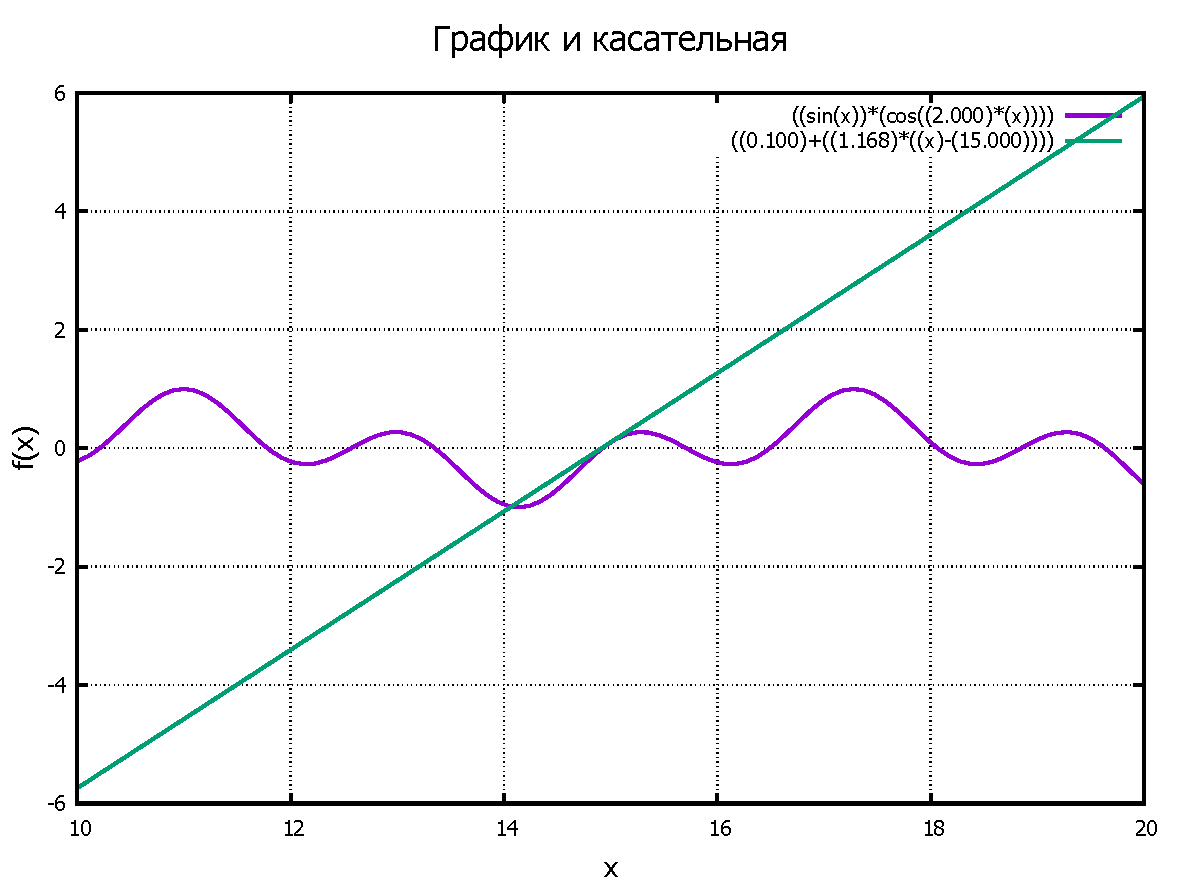
\includepdf[pages=-]{graph1.pdf}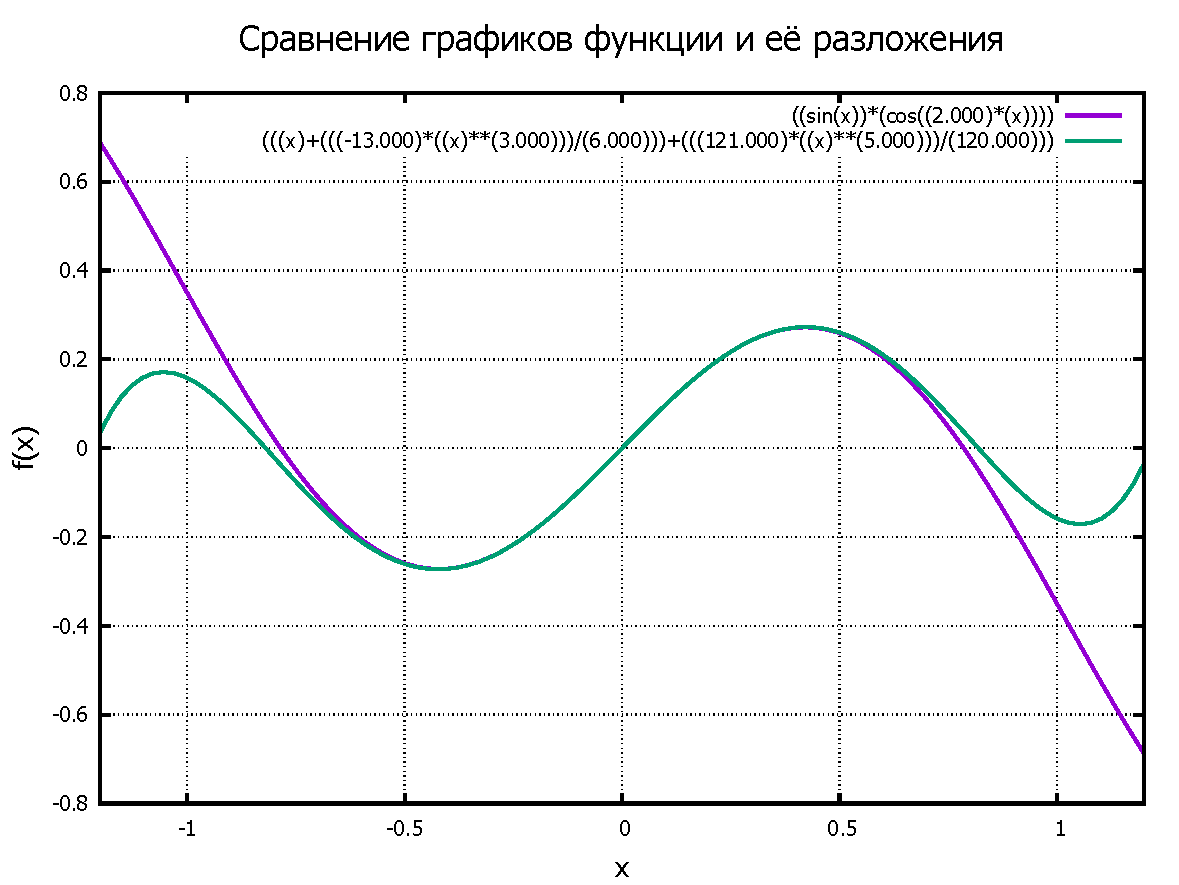
\includepdf[pages=-]{graph2.pdf}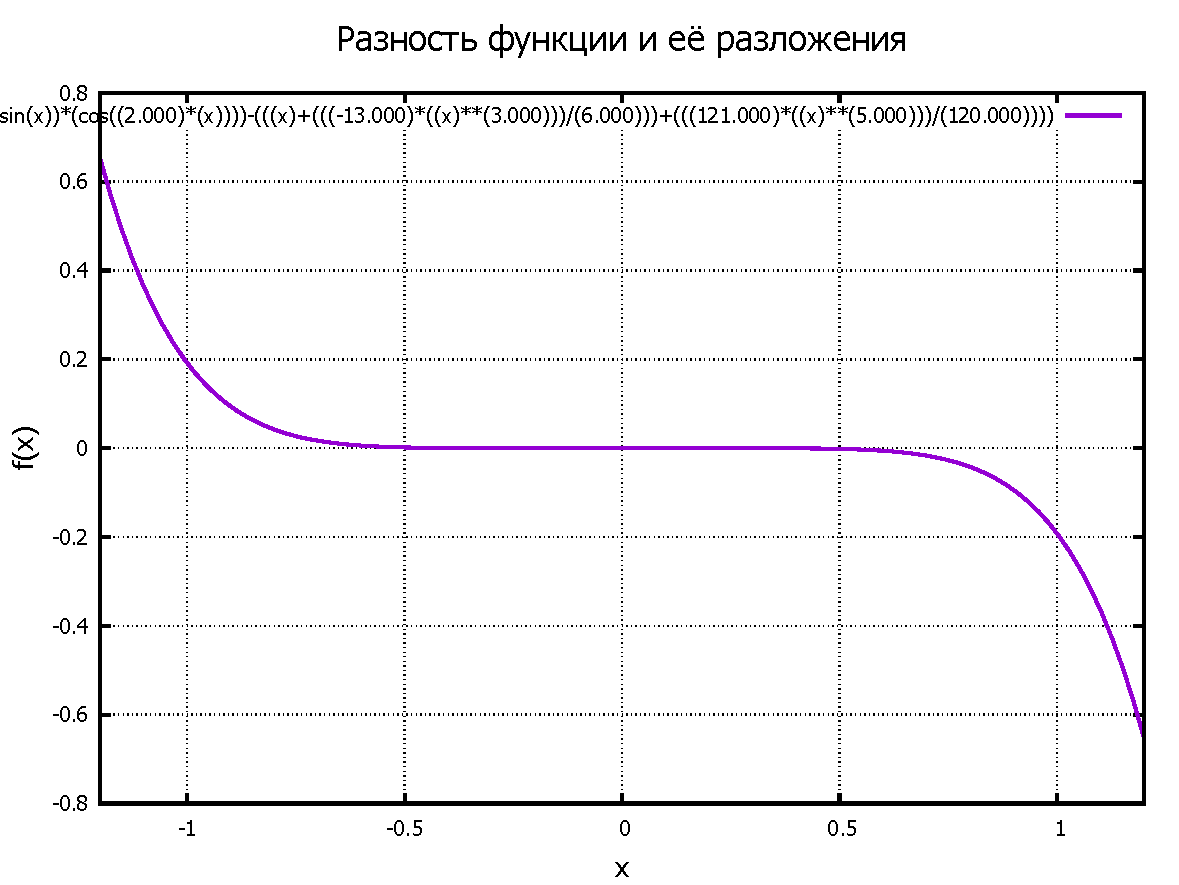
\includepdf[pages=-]{graph3.pdf}\end{flushleft}
\end{document}